\thechapter{Experimental results} 

Our system was able to produce the best results using models with higher vertex counts and smooth curves like the 
skull, while the engineer was more problematic, but increasing the vertex count also significantly increased the 
time to produce the render. Many aspects needed to be customized to particular models to get optimal results.

\begin{figure}[h]
\centering
\begin{subfigure}[b]{0.2\textwidth}
        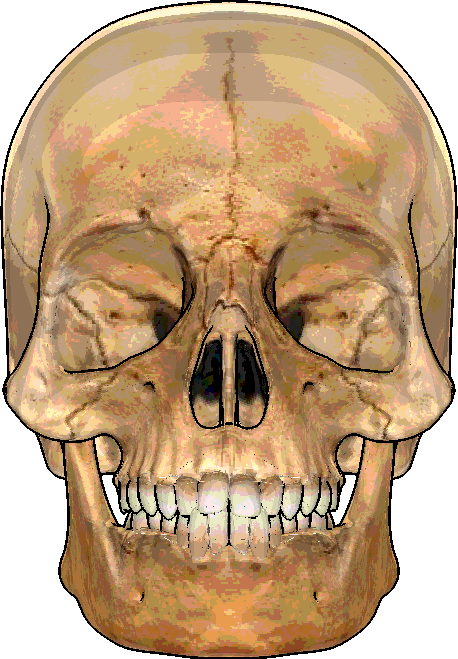
\includegraphics[width=\textwidth]{img/Combined/FinalSkull.png}
        \caption{Skull}
 		\label{fig:FinalSkull}
\end{subfigure}
~
\hspace{36pt}
~
\begin{subfigure}[b]{0.18\textwidth}
        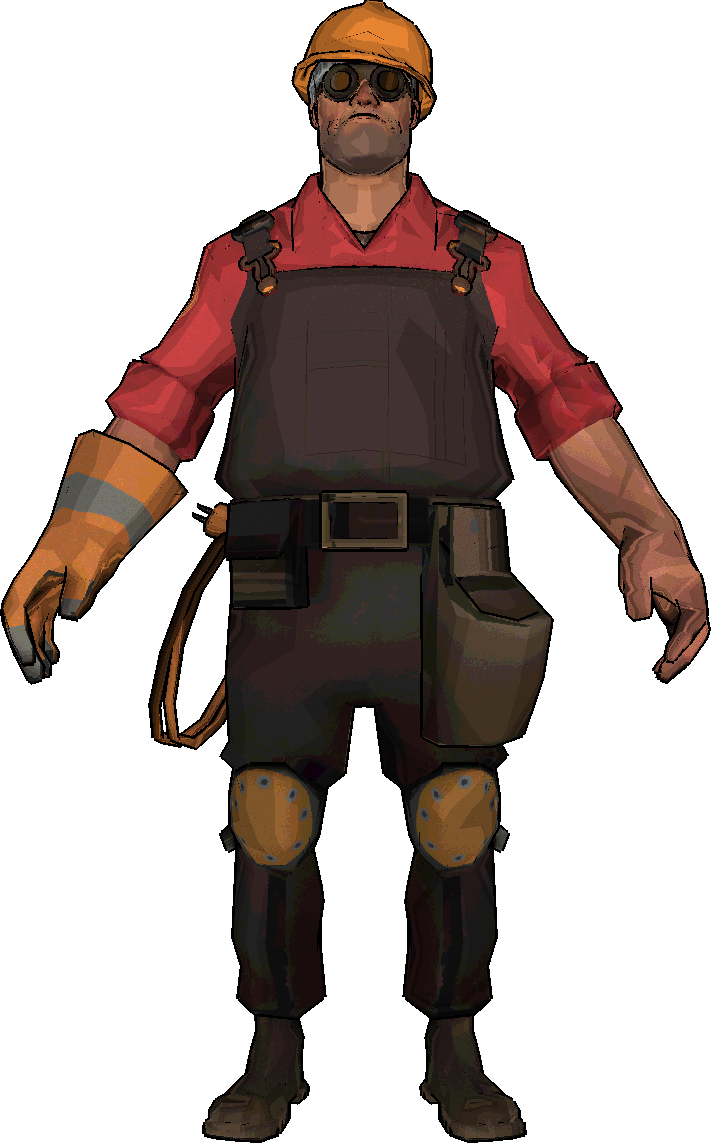
\includegraphics[width=\textwidth]{img/Combined/FinalEngineer.png}
        \caption{Engineer}
 		\label{fig:FinalEngineer}
\end{subfigure}
\caption{Final Renders}
 \label{fig:FinalRenders}
\end{figure} 

When our simple cel shading algorithm is applied to some textures the colours output need correction especially 
at lower levels as in \autoref{fig:CelShadeTexture4}, but combined with cel shaded lighting using more levels for the 
texture the desired effect can be produced as shown in \autoref{fig:FinalRenders}. 

%\begin{wrapfigure}{r}{0.5\textwidth}
\begin{figure}[h]
\centering
\begin{subfigure}[b]{0.22\textwidth}
        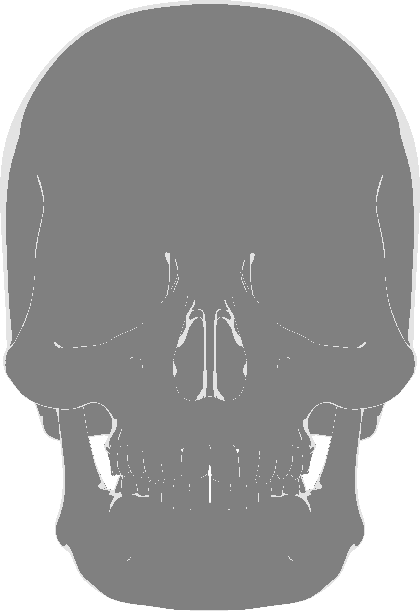
\includegraphics[width=\textwidth]{img/Lighting/Directional(0,-1).png}
        \caption{$p=(0,0,-1)$}
        \label{fig:LightingPosDir1}
\end{subfigure}
~
\hspace{24pt}
~
    \begin{subfigure}[b]{0.22\textwidth}
        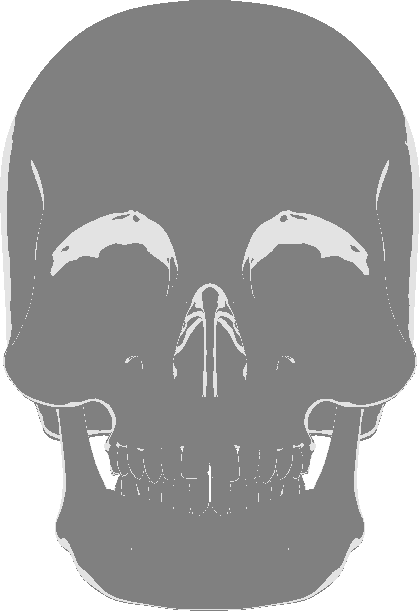
\includegraphics[width=\textwidth]{img/Lighting/Directional(10,-1).png}
        \caption{$p = (0,10,-1)$}
        \label{fig:LightingPosDir2}
    \end{subfigure}
~
\hspace{24pt}
~
    \begin{subfigure}[b]{0.22\textwidth}
        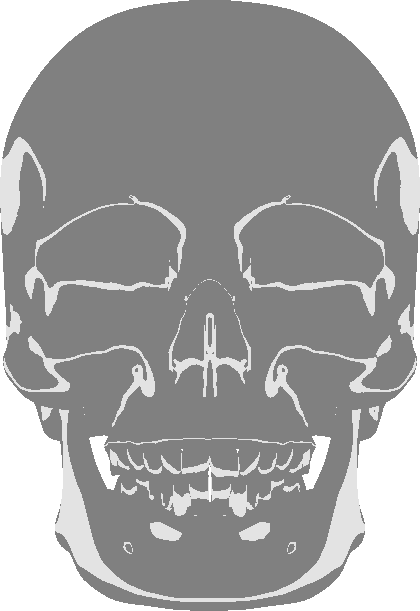
\includegraphics[width=\textwidth]{img/Lighting/Directional(100,-1).png}
        \caption{$p = (0,100,-1)$}
        \label{fig:LightingPosDir3}
    \end{subfigure}
\caption{Rim Lighting and Directional Light Position $p$}
 \label{fig:LightingPosRim}
 \end{figure}
%\end{wrapfigure} 

Positioning of the light for optimally rending the lighting is highly dependant on the model, and the area of 
the model that is being viewed. Depending on the positioning of the lighting the effect can vary greatly, 
demonstrated in \autoref{fig:LightingPosRim} where the rim lighting on the model appears dramatically different 
depending on the direction of the lighting, with differing lighting directions highlighting different areas optimally.

Close inspection of the models rendered in our system reveals some strange artifacts from the contour stage. These 
artifacts are shown in \autoref{fig:z-fighting}. The artifacts often appear as coloured line segments in the interior 
surfaces of the models. The are especially noticeable in high detail areas, or in areas where there are polygon inside 
the model. In \autoref{fig:z-fighting-high}, the effect is very noticable around the model's mouth and jaw area. 
However, in \autoref{fig:z-fighting-low}, the artifact is only noticeable in the handle of the lid. When contours are 
not drawn, the artifacts disappear. This issue is likely caused by z-fighting, which is a known limitation of depth 
buffers.

\begin{figure}[h]
    \centering
    \begin{subfigure}[b]{0.35\textwidth}
        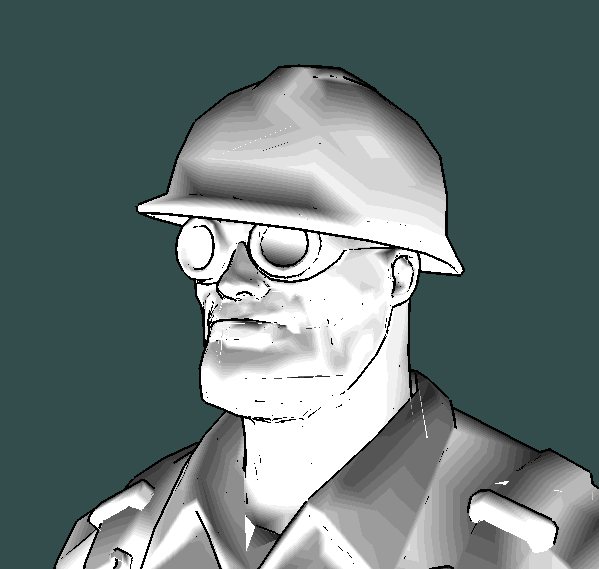
\includegraphics[width=\textwidth]{img/z-fighting-engineer}
        \caption{High detail, interior polygons}
        \label{fig:z-fighting-high}
    \end{subfigure}
    ~
    \begin{subfigure}[b]{0.35\textwidth}
        
\includegraphics[width=\textwidth]{img/z-fighting-teapot}
        \caption{Low detail, mostly convex}
        \label{fig:z-fighting-low}
    \end{subfigure}
    \caption{Artifacts caused by z-fighting}
    \label{fig:z-fighting}
\end{figure}

The depth buffer discards polygons that are completely obscured by other polygons, which allows one to tell OpenGL 
what to draw, without having to worry about the order. The depth buffer works by comparing the distance from the viewer, or 
the z-value. However, when the z-value of two polygons are very close, the z-buffer may lack the precision to be able to 
determine which pixels should be drawn, so a mix of both is drawn. This seems like a plausible explanation for why there are 
strange artifacts occurring in the renders, since all polygons are drawn, but the filled polygons are offset by a constant 
amount, so some pixels are bound to be very close to each other. Unfortunately, there isn't any easy fix for this problem. 
One solution is to not draw the polygons so close together, but this is not feasible with the current approach.
